\chapter[Solução Proposta]{Solução Proposta}


\section{Dimensionamento do Forno}

O forno de tratamento térmico possuirá um volume interno de aproximadamente 8 litros, pois o objetivo é fabricar um forno de tratamento para fins acadêmicos, com corpos de prova segundo a norma ABNT 10611 e componentes mecânicos de pequeno porte, como engrenagens.

A parte externa será compostas por uma estrutura de aço carbono como um chassi de sustentação ao peso do forno bem como todo suporte para materiais elétricos/eletrônicos, esse envoltório também será usado em formato de placas de para cobrir os tijolos expostos ao ambiente externo a fim de proteger contra choque mecânicos, conforme demonstrado no anexo b.

Os tijolos utilizados para tal construção possuem dimensões de $350 x 150 x 60$ (mm) e são próprios para suportar temperaturas superiores a $1200 \degree C$ conforme mostrado na tabela a seguir, concedida pela empresa fornecedora desse material.

\begin{figure}[h]
	\centering
	\label{tabela_dimensoes}
	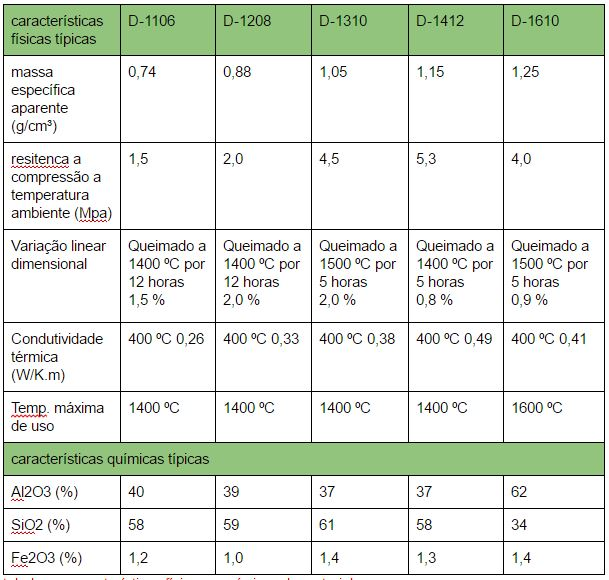
\includegraphics[keepaspectratio=true,scale=1.0]{figuras/tabela_dimensoes.JPG}
	\caption{Características físicas e químicas do material.}
\end{figure}

\subsection{Definindo alguns parâmetros de medida dentro do forno para definir os requisitos não funcionais}

Como ponto de partida, foi considerado um forno pequeno para o tratamento térmico de um corpo de prova de aço. Este corpo de prova será submetido a uma temperatura de $1200 \degree C$, afim de se introduzir a martensita em sua estrutura, que é responsável pelo endurecimento e aumento da rigidez na estrutura do aço.

Para o forno térmico, será então calculado algumas propriedades técnicas de funcionamento do forno, a espessura do isolante térmico selecionado, a temperatura máxima de operação da parede interna, onde as resistências serão instaladas, a temperatura máxima nas paredes sem a fonte de calor instalada, ou seja, várias incógnitas muito importantes na hora da montagem do produto.

A seguir é apresentado em uma tabela algumas constantes consideradas para a primeira análise dessas propriedades. Na qual estão presentes alguns valores necessário para o cálculo das propriedades previstas no parágrafo anterior.

\begin{figure}[!ht]
	\centering
	\label{tab_constantes}
	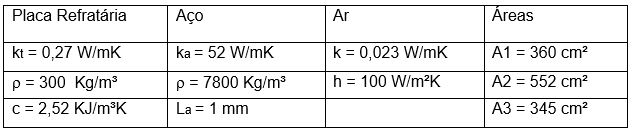
\includegraphics[keepaspectratio=true,scale=1.0]{figuras/tab_constantes.JPG}
	\caption{Tabela de propriedades técnicas.}
\end{figure}

\begin{figure}[!ht]
	\centering
	\label{vol_interno}
	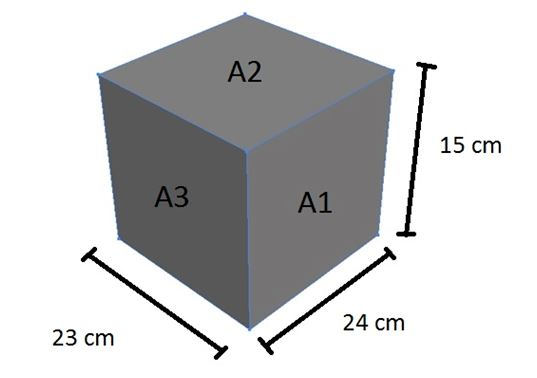
\includegraphics[keepaspectratio=true,scale=1.0]{figuras/vol_interno.JPG}
	\caption{Dados do Volume Interno do Forno.}
\end{figure}

A imagem acima retrada o dimensionamento interno escolhido pelo grupo de trabalho, onde A3 será a entrada do forno e terá área igual ao fundo, A1 e A2 são os lados, base e fundo respectivamente.

\section{Cálculo da distribuição de temperatura no interior do forno}

Nesta seção será tratado sobre os mecanismos básicos da condução de calor, convecção e condução. Estes ocorrem dentro do forno, através principalmente pela diferença de temperatura entre o interior do forno e o meio ambiente, que geram um fluxo de calor na direção do mais quente para o mais frio.

O cálculo desse fluxo de calor por meio da condução e convecção se dá pelas seguintes fórmulas.

\begin{align}
	qk = \frac{T_1 - T_2}{Rk} \\
    \text{Fluxo de calor}
    \nonumber
\end{align}
\begin{align}
	Rk = \frac{L}{Ka} \\
    \text{Condução}
    \nonumber
\end{align}
\begin{align}
	Rk = \frac{1}{ha} \\
    \text{Convecção}
    \nonumber
\end{align}

\begin{figure}[!ht]
	\centering
	\label{dist_temperatura}
	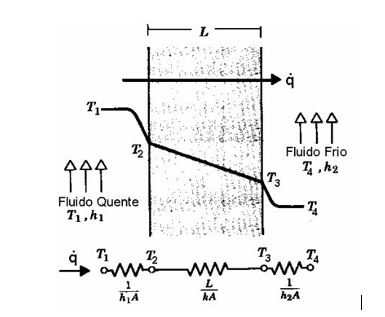
\includegraphics[keepaspectratio=true,scale=1.0]{figuras/dist_temperatura.JPG}
	\caption{Distribuição da temperatura ao longo de um material.}
\end{figure}

Com isso tudo esclarecido será calculado a temperatura nas paredes internas no forno e as espessuras da camada isolante do forno, considerando os materiais escolhidos (Tijolo refratário e o aço carbono).

Considerando o primeiro trecho, partindo do interior com 1200ºC até a parede interna com as resistências instaladas, a fórmula para o cálculo da temperatura, será apresentado logo a seguir.

Foi considerado as paredes laterais do forno, a base e o topo como tendo resistências, a temperatura nessas paredes, em A1 e A2 será a seguinte.

\begin{align}
	T1 &= 1473K + \frac{qk}{har*A1} \\
	T2 &= 1473K + \frac{qk}{har*A2}
\end{align}

Além disso foi considerado que as resistências estão igualmente espaçadas nas 4 paredes, ou seja, a potência também será dividida e sendo considerada como 750 W em A1 e A2.

\begin{align}
	T_1 &= \frac{1473 + 750} {100*360*10^{-4}} \\
	T_1 &= 1682K = 1409 \degree C
    \nonumber
\end{align}
\begin{align}
    T_2 &= \frac{1473 + 750} {100*552*10^{-4}} \\
	T_2 &= 1609K = 1336 \degree C
    \nonumber
\end{align}

As temperaturas nas supferfícies A3 (forno e porta), serão consideradas, iguais as temperaturas de operação do forno, para se adquirir um sobre dimensionamento da espessura requerida para os tijolos refratários, então T3 será igual a $1200 \degree C$. Em outras palavras, foi considerado que não há problema algum de isolamento no fundo e na porta do forno, ou seja, nenhuma energia estaria se dissipando.

Com as temperaturas nas paredes bem definidas, é possível calcular a transferência de calor nos tijolos refratários e nas placas de aço carbono, considerando apenas o fenômeno da condução.

\begin{align}
	\frac{dQ}{dt} = \frac{\Delta T}{R}
\end{align}
\begin{align}
	R = \frac{La}{Ka\, A} + \frac{Lt}{kt\, A}
\end{align}


 A única variável são as áreas que dependem da seção analisada e a espessura do tijolo. Por vias de uma segurança maior nos cálculos, serão considerados a temperatura na placa externa igual a temperatura no meio ambiente de 27ºC. A equação simplificada para obter Lt é a seguinte.

\begin{align}
    Ltx = (\Delta Tx - \frac{La}{Ka\, Ax} \frac{dQ}{dt}) \frac{kt\, Ax}{\frac{dQ}{dt}}
\end{align}

Os cálculos com os subscritos x, são correspondentes com as seções analisadas. Cada uma delas com uma área e diferença de temperaturas diferentes, e consequentemente terão espessuras requeridas diferentes. A Potência correspondente para cada seção será novamente de 750 W devido a uma divisão homogênea dos resistores nas seções consideradas.

\begin{align}
	\frac{dQ}{dt} = 750W
\end{align}

\begin{figure}[!ht]
	\centering
	\label{tab}
	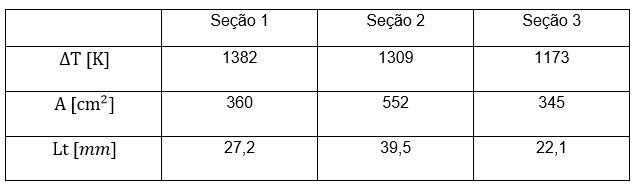
\includegraphics[keepaspectratio=true,scale=1.0]{figuras/tab.JPG}
	\caption{Cálculo das variáveis de temperatura interna do forno.}
\end{figure}

As espessuras requeridas para o tijolo refratário selecionado, foram calculadas. Este caso não leva em conta a dissipação de calor entre os tijolos. Afim de se ter tal valor, seria necessária fazer uma análise mais apurada experimentalmente ou numericamente.
Devido a todos os tipos de perdas de calor que possam ocorrer, é necessário um fator de segurança nessas espessuras obtidas.

Além disso pode ser acrescentado algum material isolante entre os tijolos e as placas externas de aço, como a vermiculita.
Por fim, também tem os sulcos que serão feitos nos tijolos para o encaixe das resistências, este fator acarretara uma perca de material refratário, sendo necessário por fins de segurança, um aumento das espessuras calculadas.

\section{Sistema de Alimentação}

\subsection{Tipo de Alimentação}

Para o funcionamento do forno de tratamento térmico foram estudadas duas formas de alimentação do sistema: 1) a gás e 2) via energia elétrica. Levando em consideração a disponibilidade e segurança, descartou-se a possibilidade da alimentação via gás, visto que o seu uso torna o sistema quanto ao manuseio periculoso, e além disso outro fator foi levado em consideração: restrição nos recursos financeiros orçados pelos alunos do projeto, e a indisponibilidade do recurso na Unidade Acadêmica de Ensino. Logo a escolha tomada para a geração de calor no forno de tratamento térmico se dará por meio da energia disponível e mais viável na execução do projeto: a energia elétrica.

Como requisitos de segurança do sistema e da rede que conecta a tomada, o sistema será dimensionado para até 15 Amperes de corrente, pois de acordo com a NBR 14136, as tomadas domésticas devem operar a uma corrente de até 20 Amperes. Fazendo um fator de segurança de 5 Amperes evitamos vários problemas com a sobre carga do circuito

\subsection{Sistema de Aquecimento}

Para que o interior do forno de tratamento térmico atinja altas temperaturas (até $1200 \degree \text{C}$), serão usados resistores para a geração de calor, os quais serão conectados a fonte de tensão a partir de um circuito de controle de corrente e estarão posicionados nas paredes internas do forno. Tais resistores se comportarão como fontes de calor para atmosfera interna do forno, e estarão dispostos de forma que tenha a maior área possível de contato para o ar e que exista um caminho livre para circulação e transferência do calor.

\subsection{Cálculo de Potência e Tempo de Aquecimento}

Para alcançar a potência desejada de 3kW dimensionou-se as propriedades termodinâmicas no volume de controle do forno.

Para definir a Potência, julgou-se uma situação de alta quantidade de calor necessária para esquentar um corpo de prova cujo tamanho seja igual ao volume interno do forno e de temperatura de têmpera alta, próxima ao definido pelo escopo do projeto que é um forno que atinja $1200 \degree \text{C}$. O material escolhido foi o Aço rápido sinterizado ASP 2017. Segue abaixo a curva de transformação com resfriamento contínuo do aço citado [11].
\begin{figure}[!ht]
	\centering
	\label{transf_continuo}
	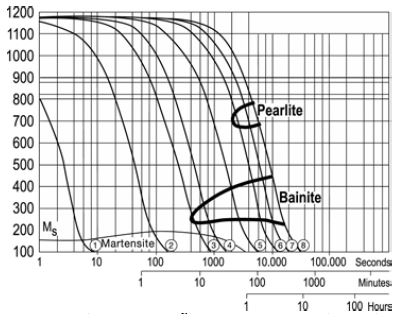
\includegraphics[keepaspectratio=true,scale=0.8]{figuras/transf_continuo.JPG}
	\caption{Curva de transformação com resfriamento contínuo.}
\end{figure}

\begin{align}
	T_{temp} = 1180 \degree \text{C}
\end{align}

A quantidade de calor necessária para aquecer a temperatura de têmpera do Aço rápido sinterizado ASP 2017 está diretamente relacionada às suas propriedades como $T_{temp} = 1180 \degree \text{C}$, sua massa específica $p = 8000 kg/m^{3}$ e seu calor específico $c = 420 J/Kg \degree C$ (Referência) não variando com a Temperatura, pela fórmula abaixo:

\begin{align}
	Q = \rho * V * c * (T_{temp} - T_{amb})
\end{align}

Sendo V o volume de aproximadamente 8,28 litros, a $T_{amb}=20 \degree C$, substituindo na fórmula temos:

\begin{align}
Q &= 8*10^{3}*8,28*10^{-3}*420*(1180-20) \\
\nonumber
Q &= 32,3 MJ
\end{align}

A partir dessa proposição e de acordo com a Primeira Lei da Termodinâmica para balanço de energia, e considerando o sistema adiabático de dentro do forno para o meio externo, a quantidade de calor Q é igual ao trabalho elétrico Wel convertido em energia térmica no meio. Sendo assim o balanço de energia se dá como:

\begin{align}
Q &= W_{el}
\end{align}

Possuindo o Wel, conseguimos relacionar a Potência necessária para o forno, através da fórmula:

\begin{align}
P &= \frac{W_{el}}{\Delta t}
\end{align}

Sendo P a potência e $\Delta t$ o tempo em segundos.

Supondo uma Potência de 3 kW, e achando o tempo necessário:

\begin{align}
\Delta t &= \frac{W_{el}}{P} = \frac{32,3*10^6}{3*10^3} = 10758s = 2,98h
\end{align}

Portanto, para aquecer um corpo de prova em uma situação de alta exigência do forno, o tempo de 3 horas é julgado aceitável para o projeto.

\subsection{Dimensionamento da Resistência Elétrica}

Para calcular a resistência foi utilizada a seguinte fórmula:

\begin{align}
R = \frac{V^2}{P}
\end{align}

Em que a tensão utilizada é de 220V e a potência é de 3kW. Feito os cálculos, a resistência encontrada foi de $16,13 \Omega$. Estas serão as condições para calcular a corrente máxima, onde o forno chegará a temperaturas de $1200 \degree \text{C}$. Para o material foi escolhido o fio Kanthal A-1(Cr 22\%, Al 5.8\% e Fe 72.2\%), levando em consideração a durabilidade e o alto desempenho desse material. Sabendo que o valor da resistência varia de acordo com a temperatura, é necessário converter essa resistência de acordo com a temperatura ambiente. Para valores de corrente e resistência, utilizou-se a temperatura de $20 \degree C$, da seguinte forma:

\begin{align}
R = \frac{R(T)}{C_T(T)}
\end{align}

Onde $R(T)=16,13\Omega$ e $C_{T}(T)=1,04$, que é o fator de conversão do material a $1200\degree \text{C}$. Obtendo $R_{20\degree \text{C}}=16,78\Omega$.
A corrente máxima que passa através do fio é dada por:

\begin{align}
I_{M\acute{A}X} = \frac{V}{R}
\end{align}

Utilizando $V=220V$ e $R=16,13\Omega$ , obtém-se a corrente máxima de $13,64 A$ que está dentro da faixa de seguraça definida no projeto. Para escolher o fio mais apropriado que irá suportar essa corrente sem ser sobrecarregado foi calculada a superfície irradiante, que é calculada pela seguinte expressão:

\begin{align}
S_i = \frac{I_{M\acute{A}X}^{2}*C_T(T)}{\gamma}
\end{align}

Substituindo $I_{M\acute{A}X}=13,64A$, $C_T(T)=1,04$ e $y=2W/cm^{2}$(capacidade de condução de corrente), tem-se. Pelas tabelas Kanthal, o fio mais apropriado, cuja superfície irradiante se encontra mais próxima desse valor, é o fio Kanthal A-1 com diâmetro 1,80mm e resistividade de $0,546\Omega /m$. O comprimento do fio é calculado pela expressão:

\begin{align}
I= \frac{R_{20 \degree \text{C}}}{0,546}
\end{align}

O comprimento encontrado foi de 30,73m.

\subsection{Distribuição dos Resistores}

Após saber o comprimento da resistência, a potência e a energia térmica necessária podemos dimensionar a distribuição dos resistores pelo volume interno do forno. \text{C}om os 30,73 metros calculados, será comprado uma quantidade de 35 metros de comprimento já enrolado que será distribuída pelas paredes do forno.
A distribuição dependerá do tamanho final da peça a ser comprada, onde ela será acoplada as paredes a partir de canaletas furadas com um diâmetro um pouco menor que o da espiral da resistência para que ela fique bem fixa. O espaço entre as canaletas deve ser de uma distância segura entre elas como a distancia de um diâmetro da bobina. As resistências serão dispostas nas pareces laterais em formato de S em cada parede e terá seus terminais acoplados em três parafusos na parede de fundo do Forno. A ligação dos resistores com o circuito ocorrerá em paralelo, sendo os dois terminais ligados a dois parafusos na perfurados no fundo do forno que serão conectados ao circuito elétrico, e um terceiro parafuso que será enrolado com as outras extremidades das resistências transformando as duas em uma resistências só acoplada. Este parafuso não atravessará completamente o tijolo e não terá contato com a parte externa. Para segurança, uma caixa pequena de proteção será acoplada na parte traseira externa do forno para que não haja contato acidental com os parafusos e nem com o termostato.
Quando o operador tiver controle da quantidade de energia térmica do sistema ele será capaz de aquecer com eficiência um corpo de prova exposto a um tratamento térmico. Para testar a eficiência de controle térmico do forno e sua capacidade de executar um tratamento térmico será realizado uma têmpera do aço.
\begin{figure}[!h]
	\centering
	\label{parafusos}
	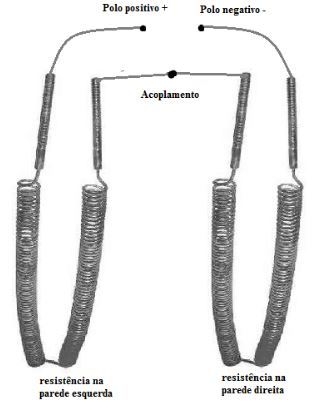
\includegraphics[keepaspectratio=true,scale=0.8]{figuras/parafusos.JPG}
	\caption{Esquema dos parafusos.}
\end{figure}

\subsection{Tratamento Térmico}

Um exemplo de tratamento térmico muito usado na industria é o processo de têmpera, que consiste no submeter o aço a uma temperatura em média $50 \degree C$ acima da zona crítica de austenitização para o aços até 0,8\% de carbono e $50 \degree C$ acima do limite inferior da zona crítica de austenitização para o aços acima de 0,8\% de carbono A zona crítica de austenitização varia com o aumento da composição de carbono no aço como na figura abaixo:
\begin{figure}[!h]
	\centering
	\label{austenitizacao}
	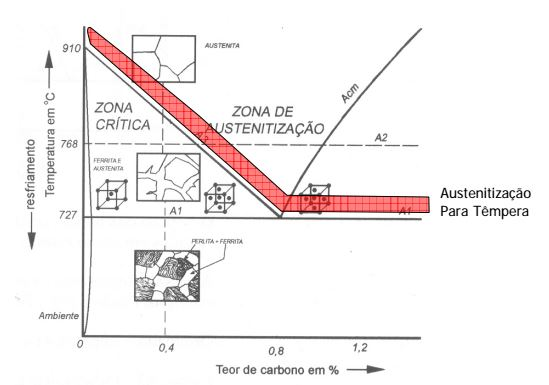
\includegraphics[keepaspectratio=true,scale=0.8]{figuras/austenitizacao.JPG}
	\caption{Zona de Austenitização para Têmpera. Fonte: Tschiptschin}
\end{figure}

Após manter o aço por um tempo  na zona crítica representada pela área vermelha do gráfico, ele muda sua sua estrutura cristalina para a austenítica ou “austenítica + cementita” que a altas temperaturas substituí qualquer estrutura existente no corpo de prova anteriormente. Após esse processo o aço é resfriado bruscamente em água passando de temperaturas entre 780 a $900 \degree C$ à temperatura ambiente de forma rápida com o objetivo de obter a estrutura Martensítica do aço que tem características duras e frágeis e evitando estruturas mais moles como ferrita, bainita e perlita:
\begin{figure}[!h]
	\centering
	\label{resfriamento1}
	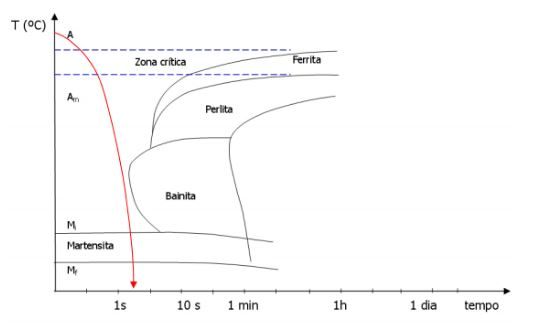
\includegraphics[keepaspectratio=true,scale=0.8]{figuras/resfriamento1.JPG}
	\caption{Resfriamento de temperatura para o processo de têmpera. Fonte: Tschiptschin.}
\end{figure}

O tempo de formação de Martensita é diferente na superfície e no centro do corpo de prova, devido ao contato direto da superfície com o meio refrigerante, levando o tempo da temperização no centro do corpo de prova a ser até 10 vezes maior que na superfície. Essa variação temporal pode gerar diferenças na estrutura do material, e isso deve ser considerado dependendo do objetivo do operador.

\begin{figure}[!h]
	\centering
	\label{resfriamento2}
	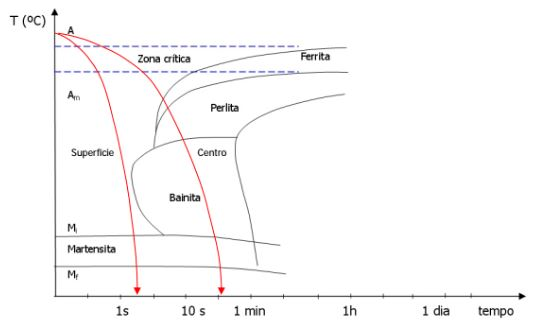
\includegraphics[keepaspectratio=true,scale=0.8]{figuras/resfriamento2.JPG}
	\caption{Resfriamento na superfície no centro do corpo de prova. Fonte: Tschiptschin.}
\end{figure}

\subsection{Material Submetido ao Tratamento}

O aço é definido no Brasil pela NBR 6215:2011 como uma liga ferrosa passível de deformação plástica que, em geral, apresenta teor de carbono entre 0,008\% e 2,0\% na sua forma combinada e, ou, dissolvida e que pode conter elementos de liga adicionados, ou residuais.

No Brasil, a Associação Brasileira de Normas Técnicas - ABTN, por intermédio da norma NBR NM 87:2000 classifica os aços-carbono comuns e os de baixo teor em liga segundo os critérios adotados pela AISI (\textit{American Iron and Steel Institute}) e SAE (\textit{Society of Automotives Engineers}).

\begin{figure}[!h]
	\centering
	\label{tab_sae1}
	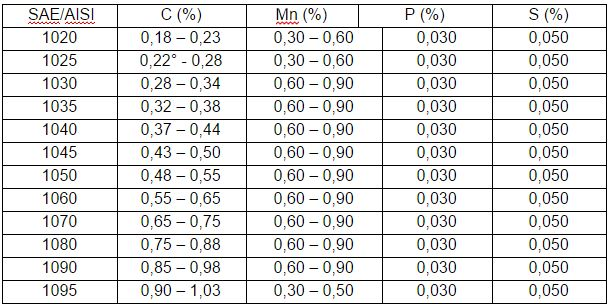
\includegraphics[keepaspectratio=true,scale=0.8]{figuras/tab_sae1.JPG}
	\caption{Composição química de aços Sae 10XX\@. Fonte: ABNT/SAE J403, 1995.}
\end{figure}

\begin{figure}[!h]
	\centering
	\label{tab_sae2}
	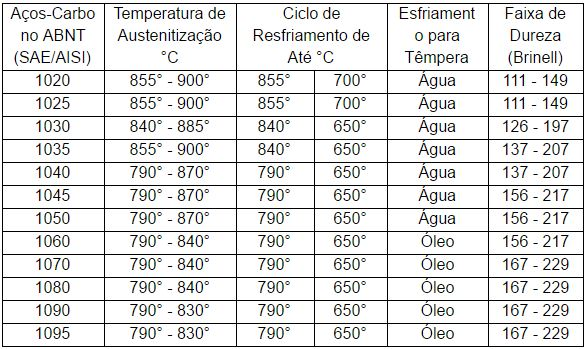
\includegraphics[keepaspectratio=true,scale=0.8]{figuras/tab_sae2.JPG}
	\caption{Características de tratamento térmico de aços-carbono simples.  Fonte: ABNT/SAE J403, 1995.}
\end{figure}

Aços são considerados bons para serem temperados a partir de 40\% de carbono em sua composição, pois possuem resistência suficiente ao desgaste a abrasão e boa tenacidade.

Para o trabalho foi escolhido o corpo de prova SAE 1045, que é considerado aço de médio teor de carbono, por questões de preço, disponibilidade, esfriamento em água facilitado e faixa de dureza próxima à aços com maior porcentagem de carbono.
São aços que possuem boa conformabilidade à frio e razoável resistência mecânica com acabamento laminado, trefilado ou retificado.

Para que seja realizados tratamentos térmicos, é necessário ter conhecimento sobre a curva TTT (tempo-temperatura-transformação) do material, que relaciona as variáveis da micro estrutura com o tempo e a temperatura.
\begin{figure}[!h]
	\centering
	\label{diagramattt}
	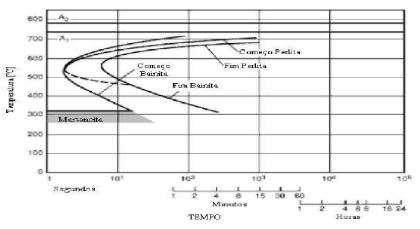
\includegraphics[keepaspectratio=true,scale=0.8]{figuras/diagramattt.JPG}
	\caption{Diagrama TTT do aço SAE 1045 Fonte: DOMINGUES et.al 2010.}
\end{figure}

\begin{figure}[!h]
	\centering
	\label{curva_temperatura}
	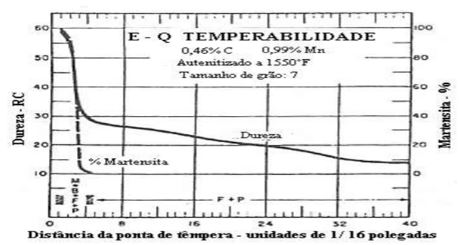
\includegraphics[keepaspectratio=true,scale=0.8]{figuras/curva_temperatura.JPG}
	\caption{Curva de temperabibilidade do aço SAE 1045. Fonte: MARTINS, 2002.}
\end{figure}

O aço Sae 1045 costuma ter no máximo seção transversal de no máximo 60mm. Para seções transversais maiores, o material não apresenta boa reação à têmpera e sua dureza diminui sensivelmente. O aço SAE 1045 deve ser aquecido entre $820 \degree C$ e $840 \degree C$ em média, por 10 minutos por milímetro, para que haja maior elevação da ductilidade e resistência assim como evitar trincamentos.

O processo de têmpera é completo após a técnica de resfriamento do material, após a temperatura de austenitização, no qual objetiva-se a formação de constituintes resultantes como cementita, ferrita e principalmente martensita, fase metaestável supersaturada de carbono e, portanto de alta dureza. O rápido processo de troca de ambiente de alto calor para um ambiente de baixo calor (até um segundo) permite a formação de martensita.

\begin{figure}[!h]
	\centering
	\label{tab_valoresH}
	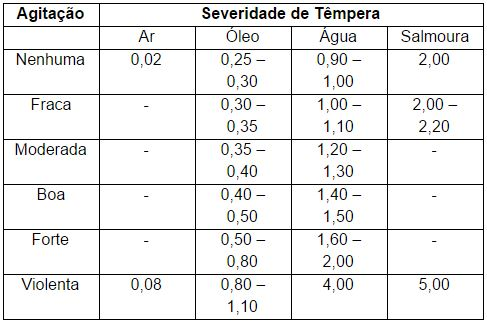
\includegraphics[keepaspectratio=true,scale=0.8]{figuras/tab_valoresH.JPG}
	\caption{Valores de H (coeficientes de severidade de têmpera) para diferentes meios de têmpera. FONTE: SCHEIDEMANTEL, 2014}
\end{figure}

A variação da taxa de resfriamento entre água e salmoura é de 27,6\% até 110\% e a diminuição do tempo de resfriamento é de 7,8\% até 63,3\% em relação à agitação. Ar e óleo possui uma severidade muito baixa de tempera e salmoura possui uam severidade mais alta que o ideal. Dessa forma o resultado de têmpera com resfriamento em água gera um aumento de 20\% de martensita na estrutura do aço em relação á tratamento com salmoura. (CARVALHO, 2004)

\section{Sistema de Controle}

O sistema de controle do forno será constituído por um conjunto de módulos de hardware e software em malha fechada, ou seja, as informações de saída influenciam no comportamento interno do sistema. O software será responsável pela interação do usuário com o forno, no qual o usuário irá determinar a temperatura de atuação desejada. Já o hardware será responsável por controlar as grandezas do sistema como corrente, tensão, temperatura.

\begin{figure}[h]
	\centering
	\label{diagrama}
	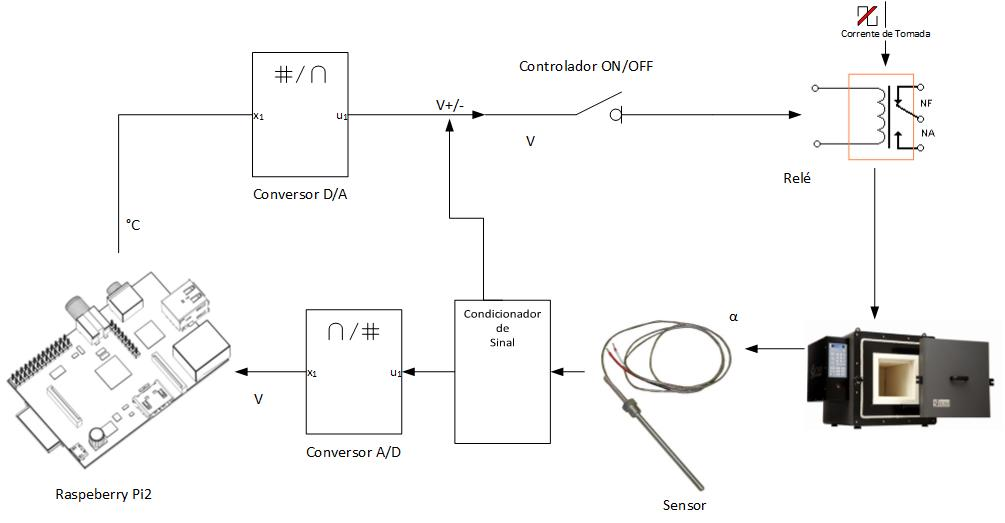
\includegraphics[keepaspectratio=true,scale=0.5]{figuras/diagrama.jpg}
	\caption{Sistema de controle de temperatura do forno}
\end{figure}

O módulo da Raspberry Pi será responsável por gerenciar um sistema de cadastro de usuários, onde por meio de seu login pessoal será possível a utilização do forno. Esse sistema registrará por meio de log de eventos, as ações realizadas no forno por este usuário específico.

Além disso, esse sistema será o responsável por dispor relatórios com os acontecimentos do experimento realizado como gráfico de tempo X temperatura. Estes relatórios serão salvos em um banco de dados, com o intuito do usuário poder consultar os seus experimentos e de outros usuários que possam ter sido feitos anteriormente, tendo assim um histórico de experimentos.

Devido as especificações técnicas dadas, o sensor termopar tipo K foi escolhido, já que possui uma grande amplitude de atuação (valores típicos entre $-270 e 1230 \degree C$). O termopar gera uma diferença de potencial de acordo com a variação de temperatura devido as características de seu material. Com isso, para iniciar o controle da temperatura do forno, inicialmente deve-se fazer uma calibração do termopar. Essa etapa consiste em determinar os valores de tensão de saída do termopar para temperaturas específicas com o intuito de se obter a relação tensão X temperatura.

Para que a temperatura do termopar possa ser obtida de maneira adequada, um circuito de amplificação será utilizado para que o seu sinal, que tem uma variação padrão de aproximadamente $41 V/ \degree C$, possa ter uma diferença significante para a resolução do conversor A/D. Esse circuito também é responsável por uma compensação de junção fria, necessária para retirar a temperatura ambiente do cálculo da temperatura.

Por fim, a tensão final é amostrada na entrada do conversor AD, que estará conectado à Raspberry Pi e irá transmitir os bits referentes a tensão lida através de um canal de comunicação SPI,sincronizado pelo clock definido pela Raspberry Pi. A Raspberry Pi irá filtrar os valores de temperatura por software. Ela também é responsável por setar a temperatura desejada. Isso é realizado através do envio dos bits através dos pinos de I/O por comunicação SPI à um conversor D/A, que irá converter para a tensão desejada que irá alimentar o circuito de controle. Esse valor de tensão representa a temperatura que deve ser lida pelos sensores com o tempo.

Ao fazer o login o usuário irá determinar qual temperatura o forno deverá ser submetido. A Raspberry Pi irá emitir um sinal digital, uma sequência de bits por exemplo, que deverá ser convertido em um sinal analógico, um valor de tensão conforme a curva definida pelo termopar. Para isso deve-se utilizar um conversor D/A, no qual sua saída será encaminhada ao módulo de controle do sistema.

Para manter o sistema na temperatura desejada será utilizado um controlador ON/OFF\@. De acordo com a figura 21, tem-se que a maior variação da temperatura de austenitização é de $40 \degree C$. Essa variação irá definir uma margem de erro, diferença entre o valor máximo e o valor mínimo, que a temperatura deverá se manter. Por exemplo, caso se defina o tratamento para o aço 1040, sua temperatura de austenitização está entre $790 \degree C$ e $870 \degree C$, com a margem de erro de $40 \degree C$, a temperatura que o usuário deverá escolher para garantir a têmpera está entre $810 \degree C$ e $850 \degree C$. Na figura abaixo foi feito uma simulação de qual resposta se espera do módulo do controlador para uma temperatura de $300 \degree C$.


\begin{figure}[h]
	\centering
	\label{on_off}
	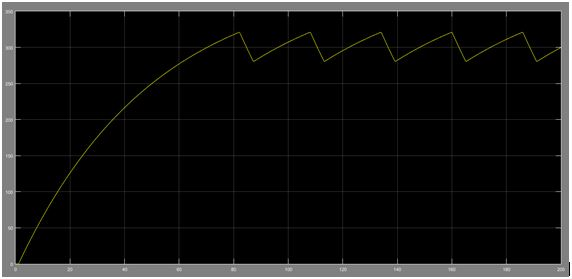
\includegraphics[keepaspectratio=true,scale=0.8]{figuras/on_off.JPG}
	\caption{Simulação do sistema utilizando um controlador ON/OFF.}
\end{figure}

A principal desvantagem do controlador ON/OFF consiste na repetida variação da saída de controle de maneira rápida e bruta, o que pode acarretar no mau funcionamento do sistema. Porém, como o forno demora um tempo considerável para atingir uma temperatura, sabe-se que esse tempo é grande o suficiente para garantir que a repetição da saída de controle será lenta, fazendo com que a saída do controlador seja feita de forma suave.

A saída do controlador irá permitir ou bloquear (ligar ou desligar) a passagem de corrente para o sistema de aquecimento do forno através de um relé. Abaixo pode-se ver o sinal de controle gerado para o mesmo sistema mostrado na figura 26.

\begin{figure}[h]
	\centering
	\label{saida_controle}
	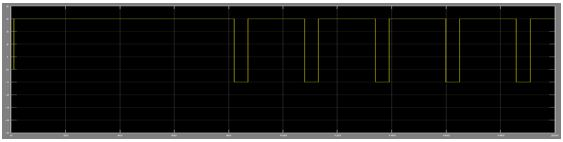
\includegraphics[keepaspectratio=true,scale=0.8]{figuras/saida_controle.JPG}
	\caption{Saída de controle do controlador ON/OFF para o relé.}
\end{figure}

\section{Arquitetura de Software}

Para a construção da aplicação proposta foi definido a implementação de um sistema web ao qual ficarão dispostas todas as funcionalidades. Este sistema terá como servidor a Raspberry Pi e múltiplos usuários poderão se conectar e visualizar o processo de têmpera.

Com isso, a implementação deste sistema utilizará das seguintes tecnologias:
\begin{itemize}
	\item Linguagem de Programação \textbf{Python} - linguagem de programação de alto nível, multiparadigma, interpretada e de tipagem dinâmica e forte;
	\item \textbf{Django Framework} - framework para desenvolvimento web, escrito em Python, open source, que utiliza o padrão model-template-view. (MTV), utiliza por padrão banco de dados Sqlite3;
	\item \textbf{REST Framework} -  ferramenta open source poderosa e flexível para a construção de APIs Web.
	\item \textbf{ReactJS} - biblioteca open source de JavaScript fornecendo uma visão para os dados processados em HTML\@. Utiliza-se do conceito de componentes, aos quais permite uma modularização da página web, diminuindo assim sua interdependência e aumentando o reuso.

\end{itemize}

\subsection{Metodologia de Desenvolvimento}

A metodologia do projeto de software do forno deverá seguir as seguintes práticas:
\begin{itemize}
	\item Elicitação de requisitos: Serão utilizados métodos de brainstorming e prototipação rápida para aquisição de novas features. Cada feature nova será escrita em um cartão com uma linguagem simples para que qualquer pessoa, sendo desenvolvedora ou não, consiga entender do que se trata. Em cada cartão haverá também valor de prioridade e critérios de aceitação para que o seja validada.
	\item Cartões: os cartões seguem dois modelos. O primeiro, criado em 2001 por uma equipe de desenvolvedores da empresa Connextra. Deve possuir título auto explicativo e a descrição seguindo o formato “Como <papel>, gostaria que <desejo/meta>, de modo que <benefício>”. O segundo é o modelo dos três C’s que foi idealizado por Ron Jeffries também em 2001. Além de conter a descrição do cartão no formato acima, juntamente com o valor de prioridade, ainda há espaços para conversação entre desenvolvedores e clientes e, por fim, os critérios de aceitação que é a confirmação de que o que foi desenvolvido está de acordo com o descrito.
	\item Kanban: ferramenta para indicar o andamento do fluxo do processo de desenvolvimento do software, permite um controle detalhado de em qual etapa se encontra a funcionalidade que esteja sendo desenvolvida. Constitui de um quadro com 4 colunas em geral: Backlog - onde ficam as funcionalidades à serem desenvolvidas; A fazer (To do) - selecionadas as funcionalidades definidas para aquela determinada Sprint, elas são colocadas nesta coluna; Em desenvolvimento (Doing) - funcionalidade em desenvolvimento; Concluída (Done) - após a finalização do desenvolvimento da funcionalidade, esta é posta nesta coluna. Assim sendo, esta ferramenta permite uma visualização melhor do fluxo de trabalho no desenvolvimento da aplicação.
	\item Sprints: é um período de tempo variável entre uma semana a um mês onde as funcionalidades escolhidas são desenvolvidas. No início de cada sprint, uma sprint planning meeting é realizada informalmente para se fazer uma retrospectiva da sprint que passou e planejamento da próxima que está começando.

\end{itemize}

\subsection{\textit{Features}}

As features do sistema de controle do forno térmico serão descritas pela matriz Feature e Benefício (FAB) \cite{safe2015}. Elas descrevem os requisitos funcionais do sistema proposto.

\begin{table}[]
	\centering
	\label{my-label}
	\begin{tabular}{|l|l|}
		\hline
		\multicolumn{1}{|c|}{\textbf{Features}}                                 & \multicolumn{1}{c|}{\textbf{Benefícios}}                                                                                                                                 \\ \hline
		\begin{tabular}[c]{@{}l@{}}Cadastro de\\   Usuários\end{tabular}        & \begin{tabular}[c]{@{}l@{}}Possibilitar o cadastro de quem\\   poderá utilizar o forno.\end{tabular}                                                                     \\ \hline
		Sistema de Login                                                        & \begin{tabular}[c]{@{}l@{}}Garantir a segurança do sistema,\\   identificando o usuário que utilizará o forno.\end{tabular}                                              \\ \hline
		\begin{tabular}[c]{@{}l@{}}Seletor de\\   Temperatura\end{tabular}      & \begin{tabular}[c]{@{}l@{}}Possibilitar ao usuário escolher a\\   temperatura desejada para a realização do experimento.\end{tabular}                                    \\ \hline
		Cronômetro                                                              & \begin{tabular}[c]{@{}l@{}}Informa o tempo decorrido do\\   experimento, o tempo esperado para término e o tempo restante para chegar no\\   esperado.\end{tabular}      \\ \hline
		\begin{tabular}[c]{@{}l@{}}Gráfico de\\   Temperatura\end{tabular}      & \begin{tabular}[c]{@{}l@{}}Apresentar ao usuário em tempo\\   real a variação de temperatura ocorrida dentro do forno.\end{tabular}                                      \\ \hline
		\begin{tabular}[c]{@{}l@{}}Iniciar\\   Processo de Têmpera\end{tabular} & \begin{tabular}[c]{@{}l@{}}Permitir ao usuário iniciar o\\   processo ao que se dará o experimento.\end{tabular}                                                         \\ \hline
		\begin{tabular}[c]{@{}l@{}}Histórico\\   de Sessão\end{tabular}         & \begin{tabular}[c]{@{}l@{}}Salvar relatório dos experimentos\\   anteriormente realizados, e apresentá-los caso solicitados.\end{tabular}                                \\ \hline
		\begin{tabular}[c]{@{}l@{}}Sistema de\\   Segurança\end{tabular}        & \begin{tabular}[c]{@{}l@{}}Dispor de um botão-emergência ao\\   qual deverá interromper o processo imediatamente.\end{tabular}                                           \\ \hline
		Informações                                                             & \begin{tabular}[c]{@{}l@{}}Mostrar informações sobre o\\   processo à de têmpera, assim como as informações necessárias para realização\\   do experimento.\end{tabular} \\ \hline
		NBRs                                                                    & \begin{tabular}[c]{@{}l@{}}Apresentar ao usuário as normas\\   relacionadas ao procedimento e materiais.\end{tabular}                                                    \\ \hline
		Estatísticas                                                            & \begin{tabular}[c]{@{}l@{}}Por meio dos dados de experimentos\\   anteriores, apresentar estatísticas sobre a utilização do forno.\end{tabular}                          \\ \hline
	\end{tabular}
	\caption{Matriz de \textit{Features}}
\end{table}